\section{Connections and curvature}

\begin{frame}{What we hope to capture and explain}
  \( \vcenter{\hbox{\includegraphics[width=30mm]{figs/curved_cube/curved_cube1}}} \!\!\to\!\! \)
  \( \vcenter{\hbox{\includegraphics[width=30mm]{figs/curved_cube/curved_cube2}}}\!\!\to\!\! \)
  \( \vcenter{\hbox{\includegraphics[width=30mm]{figs/curved_cube/curved_cube3}}}\!\!\to\!\! \)
  \( \vcenter{\hbox{\includegraphics[width=30mm]{figs/curved_cube/curved_cube4}}}\!\!\to\!\! \)
  \( \vcenter{\hbox{\includegraphics[width=30mm]{figs/curved_cube/curved_cube5}}}\!\!\to\!\! \)
  \( \vcenter{\hbox{\includegraphics[width=30mm]{figs/curved_cube/curved_cube6}}}\!\!\to\!\! \)
  \( \vcenter{\hbox{\includegraphics[width=30mm]{figs/curved_cube/curved_cube7}}}\!\!\to\!\! \)
  \( \vcenter{\hbox{\includegraphics[width=30mm]{figs/curved_cube/curved_cube8}}} \)
\end{frame}

\begin{frame}{\( T:\mm\to\EMzo \) extending \( \link \)}
We define \( T \) on edges by imaginging \alert{tipping}:

\begingroup
\tikzset{every picture/.style={scale=0.85}}
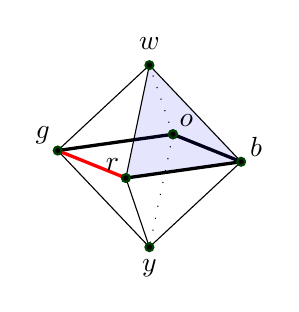
\begin{tikzpicture}%
  [x={(-0.860769cm, -0.121512cm)},
  y={(0.508996cm, -0.205391cm)},
  z={(-0.000053cm, 0.971107cm)},
  scale=1,
  eqback/.style={very thick},
  back/.style={loosely dotted, thin},
  eqedge/.style={very thick},
  edge/.style={black, thin},
  r/.style={red},
  facet/.style={fill=blue!95!black,fill opacity=0.1},
  vertex/.style={inner sep=1pt,circle,draw=green!25!black,fill=black,thick}]
\coordinate (-1, -1, 0) at (-1, -1, 0);
\coordinate (-1, 1, 0) at (-1, 1, 0);
\coordinate (0, 0, -1) at (0, 0, -1);
\coordinate (0, 0, 1) at (0, 0, 1);
\coordinate (1, -1, 0) at (1, -1, 0);
\coordinate (1, 1, 0) at (1, 1, 0);
%% Drawing edges in the back
%%
\draw[edge,eqback] (-1, -1, 0) -- (-1, 1, 0);
\draw[edge,back] (-1, -1, 0) -- (0, 0, -1.4);
\draw[edge,back] (-1, -1, 0) -- (0, 0, 1.4);
\draw[edge,eqback] (1, -1, 0) -- (-1, -1, 0);
%% Drawing vertices in the back
%%
\node[vertex] at (-1, -1, 0)     {};
%% Drawing the facets
%%
%\fill[facet] (1, 1, 0) -- (0, 0, -1.4) -- (1, -1, 0) -- cycle {};
%\fill[facet] (1, 1, 0) -- (0, 0, 1.4) -- (1, -1, 0) -- cycle {};
\fill[facet] (1, 1, 0) -- (-1, 1, 0) -- (0, 0, 1.4) -- cycle {};
%\fill[facet] (1, 1, 0) -- (-1, 1, 0) -- (0, 0, -1.4) -- cycle {};
%% Drawing edges in the front
%%
\draw[edge] (-1, 1, 0) -- (0, 0, -1.4);
\draw[edge] (-1, 1, 0) -- (0, 0, 1.4);
\draw[eqedge] (-1, 1, 0) -- (1, 1, 0);
\draw[edge] (0, 0, -1.4) -- (1, -1, 0);
\draw[edge] (0, 0, -1.4) -- (1, 1, 0);
\draw[edge] (0, 0, 1.4) -- (1, -1, 0);
\draw[edge] (0, 0, 1.4) -- (1, 1, 0);
\draw[r,eqedge] (1, 1, 0) -- (1, -1, 0);
%% Drawing the vertices in the front
%%
\begin{scope}[nodes=vertex]
\node[label=above right:\( b \)] at (-1, 1, 0)     {};
\node[label=below:\( y \)] at (0, 0, -1.4)     {};
\node[label=above:\( w \)] at (0, 0, 1.4)     {};
\node[label=above left:\( g \)] at (1, -1, 0)     {};
\node[label=above left:\( r \)] at (1, 1, 0)     {};
\node[label=above right:\( o \)] at (-1, -1, 0)     {};
\end{scope}
\end{tikzpicture}
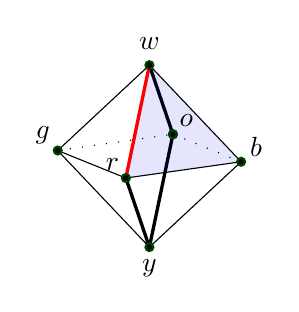
\begin{tikzpicture}%
  [x={(-0.860769cm, -0.121512cm)},
  y={(0.508996cm, -0.205391cm)},
  z={(-0.000053cm, 0.971107cm)},
  scale=1,
  eqback/.style={very thick},
  back/.style={loosely dotted, thin},
  eqedge/.style={very thick},
  r/.style={red},
  edge/.style={black, thin},
  facet/.style={fill=blue!95!black,fill opacity=0.1},
  vertex/.style={inner sep=1pt,circle,draw=green!25!black,fill=black,thick}]
\coordinate (-1, -1, 0) at (-1, -1, 0);
\coordinate (-1, 1, 0) at (-1, 1, 0);
\coordinate (0, 0, -1) at (0, 0, -1);
\coordinate (0, 0, 1) at (0, 0, 1);
\coordinate (1, -1, 0) at (1, -1, 0);
\coordinate (1, 1, 0) at (1, 1, 0);
%% Drawing edges in the back
%%
\draw[edge,back] (-1, -1, 0) -- (-1, 1, 0);
\draw[edge,eqback] (-1, -1, 0) -- (0, 0, -1.4);
\draw[edge,eqback] (0, 0, 1.4) -- (-1, -1, 0);
\draw[edge,back] (1, -1, 0) -- (-1, -1, 0);
%% Drawing vertices in the back
%%
\node[vertex] at (-1, -1, 0)     {};
%% Drawing the facets
%%
% \fill[facet] (1, 1, 0) -- (0, 0, -1.4) -- (1, -1, 0) -- cycle {};
% \fill[facet] (1, 1, 0) -- (0, 0, 1.4) -- (1, -1, 0) -- cycle {};
\fill[facet] (1, 1, 0) -- (-1, 1, 0) -- (0, 0, 1.4) -- cycle {};
% \fill[facet] (1, 1, 0) -- (-1, 1, 0) -- (0, 0, -1.4) -- cycle {};
%% Drawing edges in the front
%%
\draw[edge] (-1, 1, 0) -- (0, 0, -1.4);
\draw[edge] (-1, 1, 0) -- (0, 0, 1.4);
\draw[edge] (-1, 1, 0) -- (1, 1, 0);
\draw[edge] (0, 0, -1.4) -- (1, -1, 0);
\draw[eqedge] (0, 0, -1.4) -- (1, 1, 0);
\draw[edge] (0, 0, 1.4) -- (1, -1, 0);
\draw[r,eqedge] (1, 1, 0) -- (0, 0, 1.4) ;
\draw[edge] (1, 1, 0) -- (1, -1, 0);
%% Drawing the vertices in the front
%%
\begin{scope}[nodes=vertex]
\node[label=above right:\( b \)] at (-1, 1, 0)     {};
\node[label=below:\( y \)] at (0, 0, -1.4)     {};
\node[label=above:\( w \)] at (0, 0, 1.4)     {};
\node[label=above left:\( g \)] at (1, -1, 0)     {};
\node[label=above left:\( r \)] at (1, 1, 0)     {};
\node[label=above right:\( o \)] at (-1, -1, 0)     {};
\end{scope}
\end{tikzpicture}
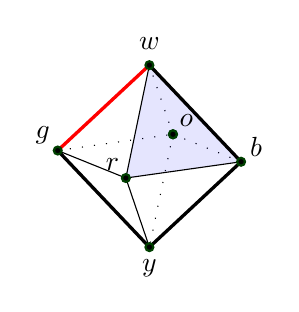
\begin{tikzpicture}%
  [x={(-0.860769cm, -0.121512cm)},
  y={(0.508996cm, -0.205391cm)},
  z={(-0.000053cm, 0.971107cm)},
  scale=1,
  eqback/.style={very thick},
  back/.style={loosely dotted, thin},
  eqedge/.style={very thick},
  r/.style={red},
  edge/.style={black, thin},
  facet/.style={fill=blue!95!black,fill opacity=0.1},
  vertex/.style={inner sep=1pt,circle,draw=green!25!black,fill=black,thick}]
\coordinate (-1, -1, 0) at (-1, -1, 0);
\coordinate (-1, 1, 0) at (-1, 1, 0);
\coordinate (0, 0, -1) at (0, 0, -1);
\coordinate (0, 0, 1) at (0, 0, 1);
\coordinate (1, -1, 0) at (1, -1, 0);
\coordinate (1, 1, 0) at (1, 1, 0);
%% Drawing edges in the back
%%
\draw[edge,back] (-1, -1, 0) -- (-1, 1, 0);
\draw[edge,back] (-1, -1, 0) -- (0, 0, -1.4);
\draw[edge,back] (-1, -1, 0) -- (0, 0, 1.4);
\draw[edge,back] (1, -1, 0) -- (-1, -1, 0);
%% Drawing vertices in the back
%%
\node[vertex] at (-1, -1, 0)     {};
%% Drawing the facets
%%
% \fill[facet] (1, 1, 0) -- (0, 0, -1.4) -- (1, -1, 0) -- cycle {};
% \fill[facet] (1, 1, 0) -- (0, 0, 1.4) -- (1, -1, 0) -- cycle {};
\fill[facet] (1, 1, 0) -- (-1, 1, 0) -- (0, 0, 1.4) -- cycle {};
% \fill[facet] (1, 1, 0) -- (-1, 1, 0) -- (0, 0, -1.4) -- cycle {};
%% Drawing edges in the front
%%
\draw[eqedge] (-1, 1, 0) -- (0, 0, -1.4);
\draw[eqedge] (0, 0, 1.4) -- (-1, 1, 0);
\draw[edge] (-1, 1, 0) -- (1, 1, 0);
\draw[eqedge] (0, 0, -1.4) -- (1, -1, 0);
\draw[edge] (0, 0, -1.4) -- (1, 1, 0);
\draw[r,eqedge] (1, -1, 0) -- (0, 0, 1.4);
\draw[edge] (0, 0, 1.4) -- (1, 1, 0);
\draw[edge] (1, 1, 0) -- (1, -1, 0);
%% Drawing the vertices in the front
%%
\begin{scope}[nodes=vertex]
\node[label=above right:\( b \)] at (-1, 1, 0)     {};
\node[label=below:\( y \)] at (0, 0, -1.4)     {};
\node[label=above:\( w \)] at (0, 0, 1.4)     {};
\node[label=above left:\( g \)] at (1, -1, 0)     {};
\node[label=above left:\( r \)] at (1, 1, 0)     {};
\node[label=above right:\( o \)] at (-1, -1, 0)     {};
\end{scope}
\end{tikzpicture}
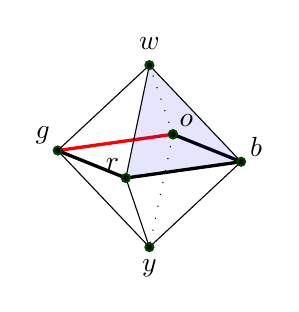
\begin{tikzpicture}%
  [x={(-0.860769cm, -0.121512cm)},
  y={(0.508996cm, -0.205391cm)},
  z={(-0.000053cm, 0.971107cm)},
  scale=1,
  eqback/.style={very thick},
  back/.style={loosely dotted, thin},
  eqedge/.style={very thick},
  edge/.style={black, thin},
  r/.style={red},
  facet/.style={fill=blue!95!black,fill opacity=0.1},
  vertex/.style={inner sep=1pt,circle,draw=green!25!black,fill=black,thick}]
\coordinate (-1, -1, 0) at (-1, -1, 0);
\coordinate (-1, 1, 0) at (-1, 1, 0);
\coordinate (0, 0, -1) at (0, 0, -1);
\coordinate (0, 0, 1) at (0, 0, 1);
\coordinate (1, -1, 0) at (1, -1, 0);
\coordinate (1, 1, 0) at (1, 1, 0);
%% Drawing edges in the back
%%
\draw[edge,eqback] (-1, -1, 0) -- (-1, 1, 0);
\draw[edge,back] (-1, -1, 0) -- (0, 0, -1.4);
\draw[edge,back] (-1, -1, 0) -- (0, 0, 1.4);
\draw[edge,eqback,r] (1, -1, 0) -- (-1, -1, 0);
%% Drawing vertices in the back
%%
\node[vertex] at (-1, -1, 0)     {};
%% Drawing the facets
%%
% \fill[facet] (1, 1, 0) -- (0, 0, -1.4) -- (1, -1, 0) -- cycle {};
% \fill[facet] (1, 1, 0) -- (0, 0, 1.4) -- (1, -1, 0) -- cycle {};
\fill[facet] (1, 1, 0) -- (-1, 1, 0) -- (0, 0, 1.4) -- cycle {};
% \fill[facet] (1, 1, 0) -- (-1, 1, 0) -- (0, 0, -1.4) -- cycle {};
%% Drawing edges in the front
%%
\draw[edge] (-1, 1, 0) -- (0, 0, -1.4);
\draw[edge] (-1, 1, 0) -- (0, 0, 1.4);
\draw[eqedge] (-1, 1, 0) -- (1, 1, 0);
\draw[edge] (0, 0, -1.4) -- (1, -1, 0);
\draw[edge] (0, 0, -1.4) -- (1, 1, 0);
\draw[edge] (0, 0, 1.4) -- (1, -1, 0);
\draw[edge] (0, 0, 1.4) -- (1, 1, 0);
\draw[eqedge] (1, 1, 0) -- (1, -1, 0);
%% Drawing the vertices in the front
%%
\begin{scope}[nodes=vertex]
\node[label=above right:\( b \)] at (-1, 1, 0)     {};
\node[label=below:\( y \)] at (0, 0, -1.4)     {};
\node[label=above:\( w \)] at (0, 0, 1.4)     {};
\node[label=above left:\( g \)] at (1, -1, 0)     {};
\node[label=above left:\( r \)] at (1, 1, 0)     {};
\node[label=above right:\( o \)] at (-1, -1, 0)     {};
\end{scope}
\end{tikzpicture}

\endgroup
\( \tr(\partial(wbr)):Tw=Tw \) is clockwise rotation by one notch.

We define \( T \) on the face \( wbr \) by the shortest homotopy \( T(wbr):\id=\tr(\partial(wbr)) \).
\end{frame}

% \begin{frame}{Rotation}
% Let \( R:\gr{abcd}\to\gr{abcd} \) send \( a\mapsto b , b\mapsto c , c\mapsto d, d\mapsto a \). \\~\\
% 
% Extend \( R \) to edges.
% 
% \begin{lemma}
% \( \hgr{R}:\hgr{abcd}\to\hgr{abcd} \) is homotopic to the identity, i.e. we have \( \pit{x:\hgr{abcd}}x=\hgr{R}(x) \).
% \end{lemma}
% \begin{proof}
% Use edges.
% \end{proof}
% \end{frame}

\begin{frame}
\begin{definition}
If \( \mm\defeq \mm_0\xrightarrow[]{\imath_0}\cdots\xrightarrow[]{\imath_{n-1}}\mm_n \) is a realization and all the triangles commute in the diagram:\vspace{-10pt}
\[\begin{tikzcd}[ampersand replacement=\&, column sep=small]
  {\mm_0} \& {\mm_1} \& {\mm_2} \& \cdots \& {\mm_n} \\
\&\& {\mathcal{U}}
\arrow["{\imath_0}", from=1-1, to=1-2]
\arrow["{f_0}", from=1-1, to=2-3]
\arrow["{\imath_1}", from=1-2, to=1-3]
\arrow["{f_1}", from=1-2, to=2-3]
\arrow["{\imath_2}", from=1-3, to=1-4]
\arrow["{f_2}", from=1-3, to=2-3]
\arrow["{\imath_{n-1}}", from=1-4, to=1-5]
\arrow["f_n"', from=1-5, to=2-3]
\end{tikzcd}\]\vspace{-15pt}
\begin{itemize}
\item The map \( f_k \) is a \defemph{\( k \)-bundle} on \( \mm \).
\item The pair given by the map \( f_k \) and the proof \( f_k\circ \imath_{k-1}=f_{k-1} \), i.e. that \( f_k \) extends \( f_{k-1} \) is called a \defemph{\( k \)-connection on the \( (k-1) \)-bundle \( f_{k-1} \)}.
\end{itemize}
\end{definition}
\end{frame}

\begin{frame}
\begin{mydef}[cont.]
\[\begin{tikzcd}[ampersand replacement=\&, column sep=small]
  {M_k\times \partial\Delta^k} \& {M_k} \\
  {\mathbb{M}_{k-1}} \& {\mathbb{M}_k} \\
  \& {\mathcal{U}}
  \arrow["{\mathrm{pr}_1}", from=1-1, to=1-2]
  \arrow["{\mathbb{A}_{k-1}}"', from=1-1, to=2-1]
  \arrow["{*_{\mathbb{M}_k}}", from=1-2, to=2-2]
  \arrow["{h_k}", shorten <=10pt, shorten >=10pt, Rightarrow, from=2-1, to=1-2]
  \arrow["{\imath_{k-1}}", from=2-1, to=2-2]
  \arrow[""{name=0, anchor=center, inner sep=0}, "{f_{k-1}}"', from=2-1, to=3-2]
  \arrow["\ulcorner"{pos=-0.05, rotate=180}, shift left=1.5, draw=none, from=2-2, to=1-1]
  \arrow["{f_k}", from=2-2, to=3-2]
\end{tikzcd}
\begin{tikzcd}[ampersand replacement=\&]
  {\{F\}\times \partial\Delta^2} \& \unit \\
  {\mathbb{M}_{k-1}} \& {\mathcal{U}}
  \arrow["{!}", from=1-1, to=1-2]
  \arrow["{\mathbb{A}_{k-1}}"', from=1-1, to=2-1]
  \arrow["{*_{\mathbb{M}_k}}", from=1-2, to=2-2]
  \arrow["{\flat_F}", shorten <=11pt, shorten >=11pt, Rightarrow, from=1-2, to=2-1]
  \arrow[from=2-1, to=2-2]
\end{tikzcd}\]
the filler \( \flat_F \) is called a \defemph{flatness structure for the face \( F \)}, and its ending path (the holonomy around the boundary) is called \defemph{the \( k \)-curvature at the face \( F \)}.
\end{mydef}
\end{frame}
\begin{frame}
With these definitions we have now achieved one of our main goals.

Without a definition of Euler characterisitc we can't prove Gauss-Bonnet.

But once we add vector fields there is a lot more to say.
\end{frame}

